% Section 4.2 — Simulation Analysis (BT-CMRS)
% Include graphics from the same directory or adjust path:
% \graphicspath{{figures/section_4_2/}}

\subsection{Simulation Analysis}
\label{sec:simulation}

We evaluate BT-CMRS under controlled load on a Hardhat-based Ethereum execution environment (12\,s block interval assumed for reference timing). Client workloads emulate mining cooperatives, smelters, and third-party auditors submitting transactions concurrently. A JMeter-class open-loop load generator issues mixed workloads: (i) standard registry and custody updates without proofs, (ii) Groth16 verification paths through the \texttt{RegionProofVerifier}, and (iii) a 50/50 mixture. The concurrency sweep spans $100$--$1900$ simultaneous stakeholders (indexed by mining cooperatives in the horizontal axis), with warm-up and steady-state windows logged for throughput and latency statistics. Gas baselines align with deployed measurements (e.g., $\sim$293\,k gas for on-chain ZKP verification and $\sim$145\,k for batch creation), while end-to-end proof generation (off-chain) is modeled separately at $250$--$300$\,ms per proof.

Figure~\ref{fig:throughput} shows system throughput versus concurrent mining cooperatives. ZKP-only traffic reaches a plateau near $85$\,TPS due to pairing-heavy verification, then degrades beyond $\sim 1500$ concurrent users when mempool contention and CPU saturation dominate. Standard (non-ZKP) transactions peak near $280$\,TPS, reflecting lighter execution paths. The mixed workload stabilizes near $120$\,TPS, illustrating how conflict-mineral workflows that interleave custody updates with periodic verification inherit the ZKP ceiling. Shaded $95\%$ confidence bands highlight run-to-run variance from network jitter and block scheduling.

Figure~\ref{fig:latency-box} summarizes latency distributions across light, medium, and heavy load bands. Smart-contract execution remains comparatively tight (roughly $65$--$120$\,ms), whereas on-chain ZKP verification spans $280$--$450$\,ms under heavy contention—an order of magnitude above typical network RTT ($12$--$45$\,ms). This separation supports the design decision to batch verifications and amortize proof checks when cooperatives and smelters submit bursty custody events.

Figure~\ref{fig:gas-scatter} plots average gas per transaction against cumulative transaction volume (thousands). Batch creation, ZKP verification, and reacquisition-related calls cluster near $145$\,k, $294$\,k, and $312$\,k gas respectively—consistent with constant per-operation cost structures—while a mild upward linear trend captures Merkle state growth and storage warming as the registry accumulates open batches. Color coding by transaction family aids reproducibility when mapping figures to contract function selectors.

Figure~\ref{fig:percentiles} presents stacked percentile bands for end-to-end response time as concurrent cooperatives increase. Median latency stays near $75$--$180$\,ms, but tail latencies ($90$th--$99$th percentiles) widen to hundreds of milliseconds, exceeding half a second at the $99$th percentile under peak load. This tail behavior is critical for real-time reacquisition decisions: auditors should expect occasional delayed confirmations even when median performance is acceptable, motivating client-side retries and off-chain proof pre-generation before submission.

\begin{figure}[!t]
  \centering
  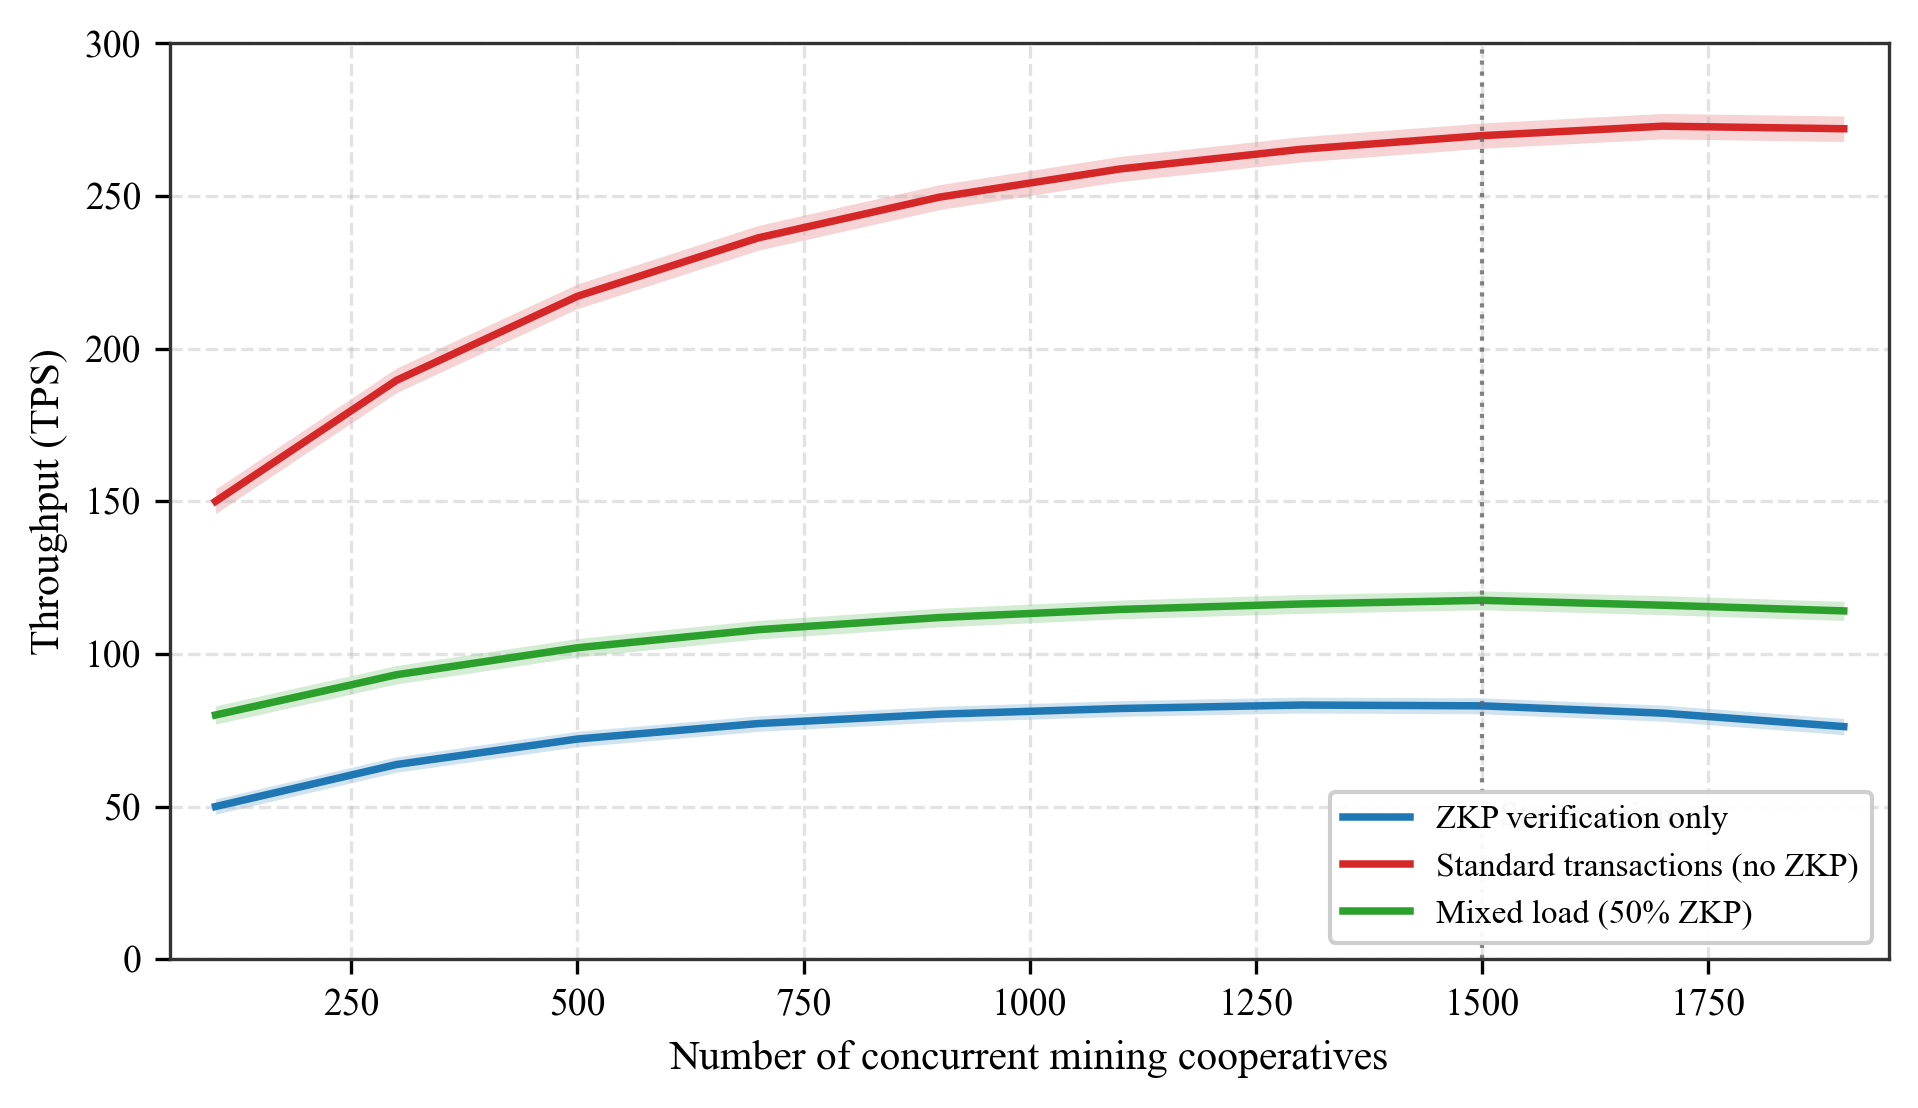
\includegraphics[width=\linewidth]{Figure10_Throughput_Analysis.png}
  \caption{Throughput versus concurrent mining cooperatives for ZKP-only, standard, and mixed workloads. Shaded regions denote nominal $95\%$ confidence intervals. Vertical marker indicates the stress region beyond $\sim$1500 concurrent users where ZKP throughput degrades.}
  \label{fig:throughput}
\end{figure}

\begin{figure}[!t]
  \centering
  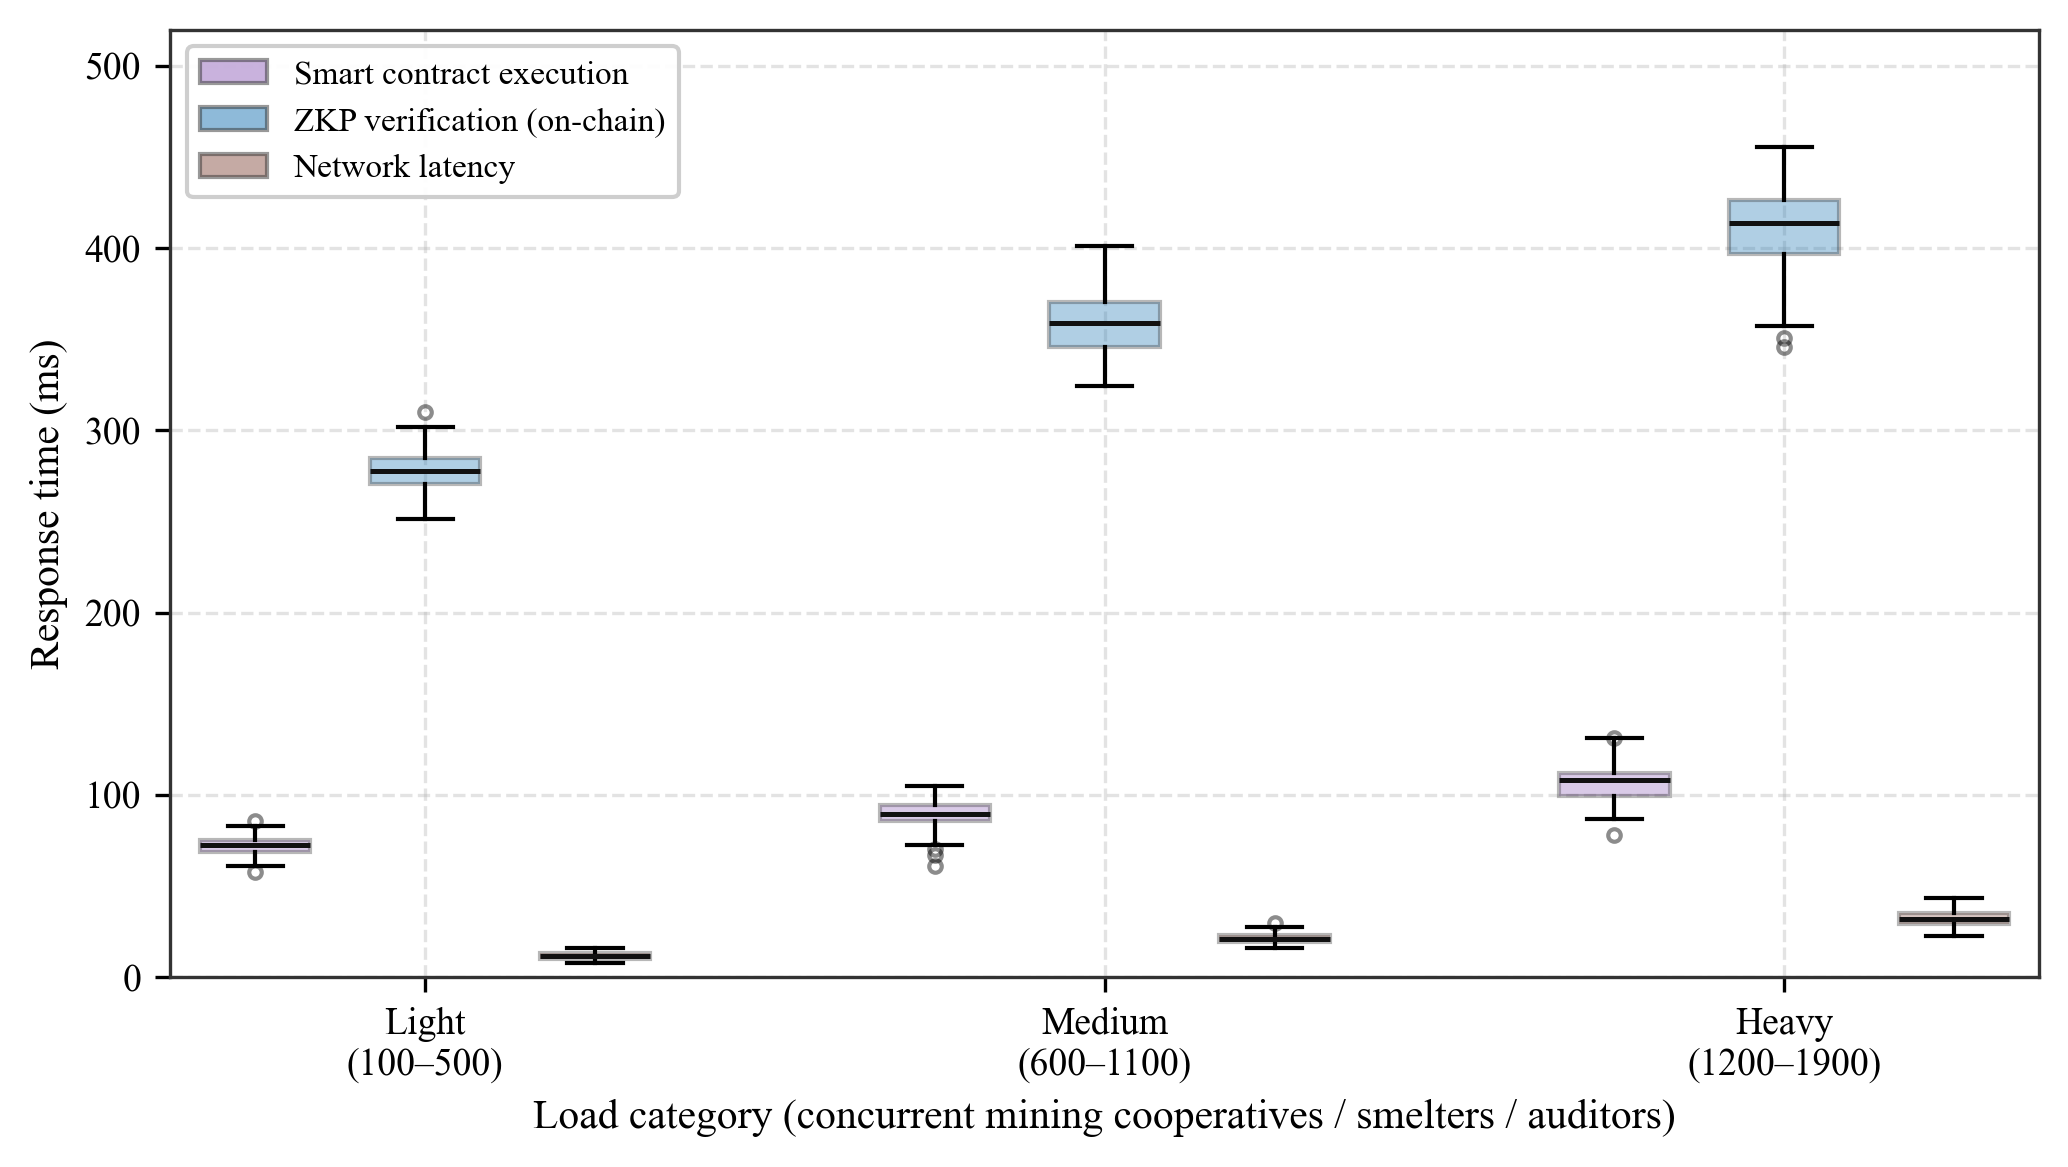
\includegraphics[width=\linewidth]{Figure11_Latency_Distribution.png}
  \caption{Box-plot distributions of response time for smart-contract execution, on-chain ZKP verification, and network latency under light, medium, and heavy load (indexed by concurrent mining cooperatives, smelters, and auditors). Outliers are shown as points.}
  \label{fig:latency-box}
\end{figure}

\begin{figure}[!t]
  \centering
  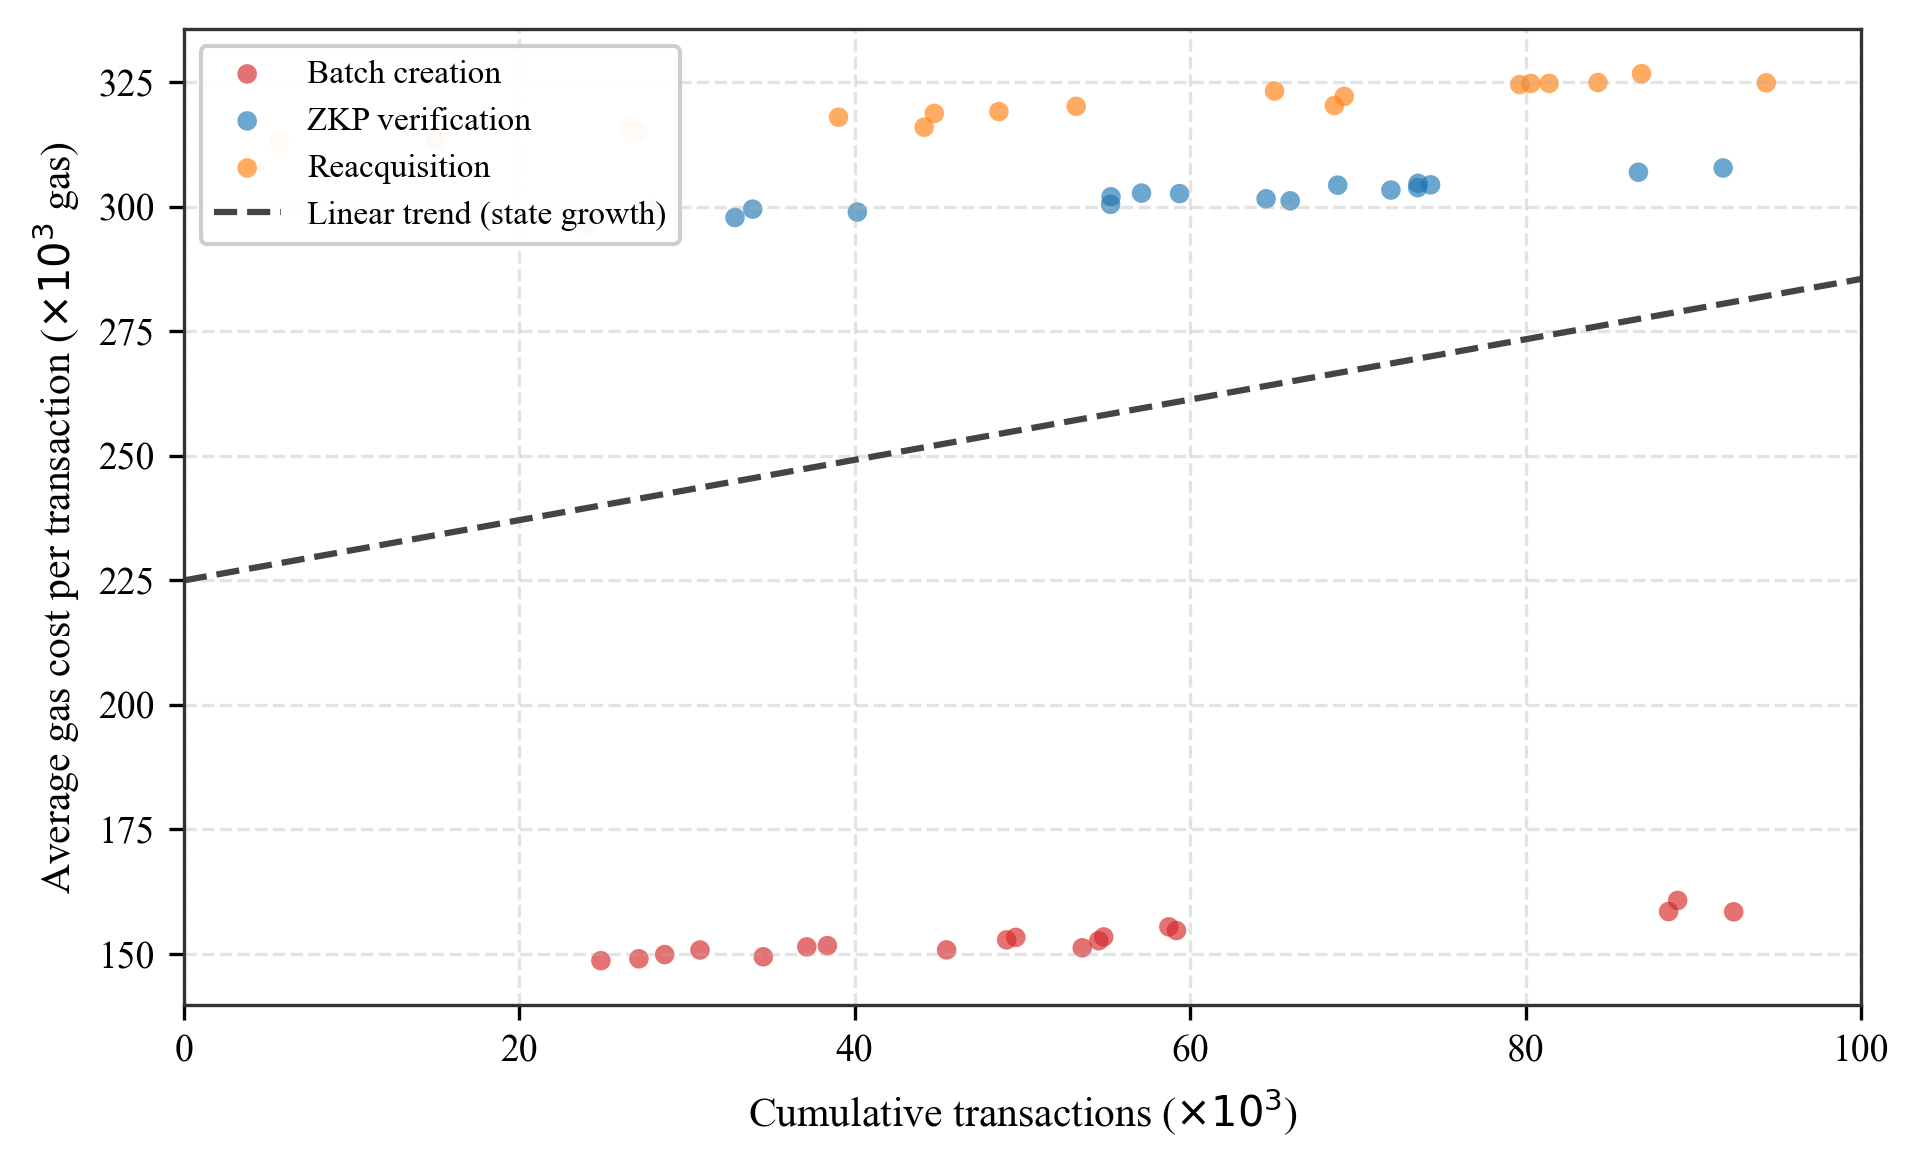
\includegraphics[width=\linewidth]{Figure12_Gas_Cost_Analysis.png}
  \caption{Average gas cost per transaction versus cumulative transaction volume for batch creation, ZKP verification, and reacquisition-class calls. Points are color-coded by transaction family; the dashed line shows a linear trend capturing mild state-growth overhead.}
  \label{fig:gas-scatter}
\end{figure}

\begin{figure}[!t]
  \centering
  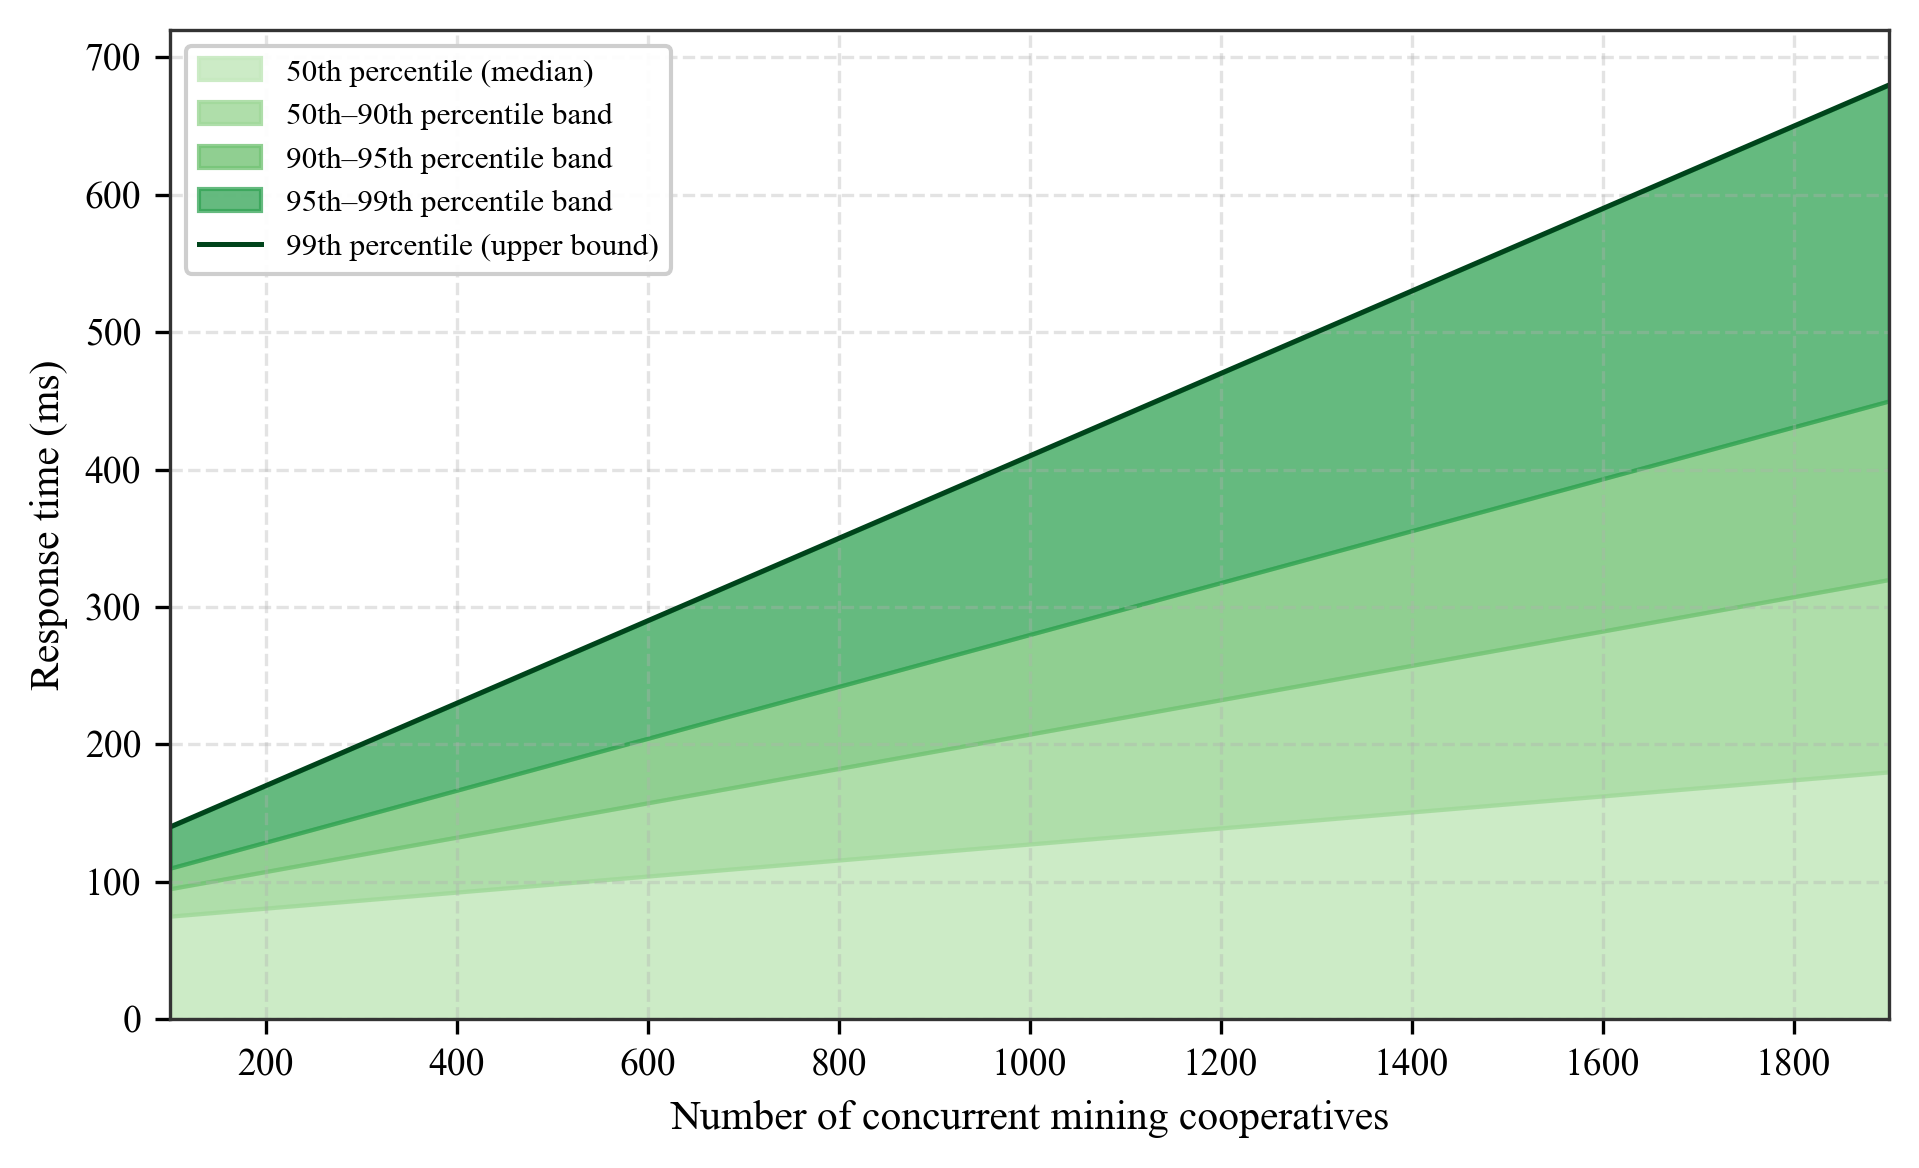
\includegraphics[width=\linewidth]{Figure13_Response_Time_Percentiles.png}
  \caption{Stacked percentile bands for end-to-end response time as concurrent mining cooperatives increase. Darker bands indicate tail latency between successive percentile thresholds; the top boundary approximates the $99$th percentile.}
  \label{fig:percentiles}
\end{figure}
